%%%%% Conference Version%%%%%%

%\documentclass[letterpaper, 10 pt, conference]{ieeeconf}



%%%% Brief Journal Paper version%%%%%
\documentclass[letterpaper, 10 pt, journal, twoside]{IEEEtran}


\usepackage{mathrsfs}
\usepackage{amssymb}
\usepackage{amsmath}
\usepackage{epsfig}
\usepackage{color}
\usepackage{booktabs}   % for \toprule / \midrule / \bottomrule in tables
\usepackage{graphicx}  % for \includegraphics
\graphicspath{{../../60_Results/}}

%%%% Selective part from steve.lib
\newcommand{\rank}{{\rm rank\;}}
\newcommand{\image}{{\rm Im\;}}
\newcommand{\stack}{{\rm stack\;}}
\newcommand{\Span}{{\rm span\;}}
\newcommand{\diag}{{\rm diag\;}}
\newcommand{\col}{{\rm col\;}}
\newcommand{\cp}{{\rm cp\;}}
\newcommand{\R}{\mathbb{R}}
\newtheorem{theorem}{Theorem}
\newtheorem{problem}{Problem}
\newtheorem{lemma}{Lemma}
\newtheorem{remark}{Remark}
\newtheorem{proposition}{Proposition}
\newtheorem{corollary}{Corollary}
\newtheorem{property}{Property}
\newtheorem{conjecture}{Conjecture}
\newtheorem{assumption}{Assumption}
\newtheorem{exercise}{Exercise}
\newtheorem{example}{Example}
\def\n{{\bf n}}
\def\m{{\bf m}}
\def\r{{\bf r}}
\def\c{{\bf c}}
\def\scr#1{{\mathcal #1}}
\def\rep#1{(\ref{#1})}
\def\eq#1{\begin{equation}#1\end{equation}}
\def\qed{ \rule{.1in}{.1in}}

%%%% Typed cross-reference macros
\newcommand{\eqnref}[1]{Eq.~(\ref{#1})}
\newcommand{\figref}[1]{Fig.~\ref{#1}}
\newcommand{\thmref}[1]{Theorem~\ref{#1}}
\newcommand{\lemref}[1]{Lemma~\ref{#1}}
\newcommand{\asmref}[1]{Assumption~\ref{#1}}
\newcommand{\probref}[1]{Problem~\ref{#1}}
\newcommand{\secref}[1]{Section~\ref{#1}}

%%%%% Redefined the \matt to avoid conflicts with the amsmatch package
\def\matt#1{\begin{bmatrix}#1\end{bmatrix}}


\title{Connectivity-Preserving V-Formation Control for Unicycle
       Multi-Robot Systems via Feedback Linearization and
       Adaptive Artificial Potential Fields}


\author{Phillipp~Gery,~\textit{ICON, Purdue University}%
\thanks{P.~Gery is with the Institute for Control, Optimization and Networks
        (ICON), Elmore Family School of Aeronautics and Astronautics,
        Purdue University, West Lafayette, IN~47907, USA.
        Course: AAE~590 Multi-Agent Autonomy and Control.}}



\begin{document}

\maketitle


%%%%%%%%%%%%%%%%%%%%%%%%%%%%%%%%%%%%%%%%%%%%%%%%%%%%%%%%%%%%%%%%%%%%%%%%%%%%%%%%
\begin{abstract}
This paper addresses decentralized formation control for a group of five
unicycle-type mobile robots navigating a cluttered two-dimensional environment
while simultaneously preserving inter-agent communication connectivity.
We extend the unified artificial potential field~(APF) framework of Kan
\emph{et al.}\ to accommodate nonholonomic unicycle kinematics through
feedback linearization via a look-ahead point transformation, which maps
each robot onto a fully actuated virtual point and enables direct application
of gradient-descent control laws.  Four novel mechanisms augment the
baseline APF architecture: (1)~a \emph{dynamic formation squeeze} that
adaptively relaxes the rigid $V$-shape geometry when navigating narrow
corridors; (2)~a \emph{saturated tangent barrier} for connectivity
preservation that applies zero force in the safe regime and grows to a
hard-capped restoring magnitude only when an inter-agent link approaches the
communication threshold; (3)~\emph{distributed target tracking} without
a single leader, enabling automatic network self-recovery after transient
topological splits; and (4)~a \emph{non-conservative vortex field}
superimposed on each obstacle's repulsion that breaks the rotational
symmetry of the conservative APF landscape, eliminating saddle-point and
local-minimum traps provably without affecting the Lyapunov energy-descent
guarantee.  A Lyapunov argument demonstrates that the safe,
connected invariant set is forward invariant under the proposed control law.
The five APF hyperparameters are tuned via Bayesian optimization over
Gaussian processes \cite{shahriari2016JMLR} across a multi-environment
gauntlet.  Simulation results in both a structured staggered gate field and
a random obstacle forest confirm successful goal acquisition, zero collisions,
and strict maintenance of $\lambda_{2}(L(t))>0$ throughout all trials.
\end{abstract}


\section{Introduction}

Coordinated multi-robot systems have attracted sustained research interest
due to their transformative potential in industrial automation, warehouse
logistics, and search-and-rescue operations \cite{wang2025RaAS}.
A fundamental capability in such systems is \emph{formation control}: the
ability to drive a group of robots into a prescribed geometric configuration
and maintain it while navigating a shared environment.
Methods based on \emph{Artificial Potential Fields}~(APF)
\cite{khatib1986IJRR,leonard2001P4ICDCCN,olfatisaber2006TAC} are
particularly attractive for their analytical tractability and real-time
implementability, unifying formation, obstacle, and connectivity objectives
in a single gradient-descent control law amenable to decentralized
implementation.

A critical requirement frequently overlooked in APF-based formation
controllers is the preservation of inter-agent \emph{communication
connectivity}.  If agents drift beyond each other's sensing range during
obstacle-avoidance maneuvers, the communication graph becomes disconnected
and cooperative control breaks down entirely.  Despite the maturity of both
APF-based formation control and nonholonomic motion planning as individual
fields, no existing work provides a unified treatment of formation
stabilization, obstacle avoidance, and connectivity preservation for
unicycle-type multi-robot systems — the platform class predominant in
warehouse and field deployments.

This paper addresses that gap with four contributions.  The primary
contribution extends the APF framework of \cite{kan2012ITAC} from point
agents to unicycle robots via feedback linearization, with a Lyapunov
stability proof.  Three additional mechanisms resolve the practical failure
modes of rigid APF architectures in highly cluttered environments: the
\emph{dynamic formation squeeze} for navigating narrow corridors, the
\emph{saturated tangent barrier} for zero-drag connectivity preservation,
and a \emph{per-obstacle vortex field} that eliminates local minima and
saddle points provably without violating the energy-descent guarantee.


\section{Related Work}

\textit{APF-based formation control.}
Artificial Potential Fields, originally proposed by Khatib
\cite{khatib1986IJRR} for single-robot navigation, were extended to the
multi-agent setting by Leonard and Fiorelli \cite{leonard2001P4ICDCCN}, who
formulated inter-agent attractive and obstacle repulsive potentials that drive
a fleet toward a desired geometric configuration.  Rimon and Koditschek
\cite{rimon1992TRA} established that such potentials can be constructed as
provably complete \emph{navigation functions} for sphere-world environments,
guaranteeing convergence from almost all initial configurations.  Ge and Cui
\cite{ge2000TRA} later addressed the ubiquitous local-minimum problem by
redesigning the repulsive term to incorporate the robot-to-goal distance,
eliminating spurious equilibria in cluttered scenes.  Olfati-Saber
\cite{olfatisaber2006TAC} extended potential-field ideas to multi-agent
flocking, providing a cohesion--separation--velocity-matching framework
that became a canonical benchmark for decentralized multi-robot design.

\textit{Communication connectivity preservation.}
The algebraic connectivity $\lambda_{2}(L)$ of the graph Laplacian $L$
provides a spectral certificate for network connectivity: the communication
graph is connected if and only if $\lambda_{2}(L)>0$ \cite{ji2007ITR}.
Ji and Egerstedt \cite{ji2007ITR} showed that connectivity maintenance can
be formulated as a hard control constraint, while Dimarogonas and
Kyriakopoulos \cite{dimarogonas2010ICTA} developed distributed controllers
that guarantee $\lambda_{2}(L(t))>0$ for all time.  Panagou
\emph{et al.}\ \cite{panagou2016ITAC} introduced smooth barrier functions
of $\lambda_{2}$ as additional potential terms, at the cost of a continuous
connectivity drag on all inter-agent motion even in the open field.

\textit{Unified APF with connectivity for point agents.}
Kan \emph{et al.}\ \cite{kan2012ITAC} represent the closest existing work,
unifying formation stabilization, obstacle avoidance, and connectivity
preservation within a single APF framework and proving convergence via a
Lyapunov argument.  That result is, however, derived exclusively for
\emph{point agents} governed by single-integrator dynamics
$\dot{p}_{i}=u_{i}$, $u_{i}\in\R^{2}$, in which the velocity vector can
be set to any direction instantaneously.  The Pfaffian nonholonomic
constraint of unicycle robots prohibits lateral velocity and fundamentally
invalidates the gradient-descent controller of \cite{kan2012ITAC}.  Do
\cite{do2008TCST} addressed formation tracking for unicycle-type robots
with limited sensing ranges, but without a connectivity-preservation
mechanism.  The present work closes this gap by combining all three
objectives for the first time in the unicycle setting.


\section{Problem Formulation}

The system consists of $N=5$ unicycle robots operating in a planar warehouse
environment with static obstacles.  We formalize the agent kinematics,
environment, inter-agent communication topology, desired formation, potential
function, and control objectives.

%-----------------------------------------------------------------------
\subsection{Agent Kinematics and State Space}
%-----------------------------------------------------------------------

Let $\scr{I}=\{1,\ldots,N\}$ index the robot fleet.  Robot $i\in\scr{I}$ is
modeled as a unicycle (differential-drive) agent with configuration
$\mathbf{q}_{i}=[x_{i},\,y_{i},\,\theta_{i}]^{\top}\in\R^{2}\times S^{1}$,
where $(x_{i},y_{i})$ is the Cartesian position and
$\theta_{i}\in(-\pi,\pi]$ is the heading angle.  The continuous-time kinematics
are
\begin{equation}
  \dot{x}_{i}=v_{i}\cos\theta_{i}, \quad
  \dot{y}_{i}=v_{i}\sin\theta_{i}, \quad
  \dot{\theta}_{i}=\omega_{i},
  \label{eq:unicycle}
\end{equation}
where $v_{i}\in\R$ and $\omega_{i}\in\R$ are the linear and angular velocity
inputs, respectively.  Let $p_{i}=[x_{i},\,y_{i}]^{\top}\in\R^{2}$ denote the
planar position of agent $i$ and define the stacked position vector
$\mathbf{p}=\stack_{i\in\scr{I}}p_{i}\in\R^{2N}$.

The unicycle is subject to the Pfaffian nonholonomic constraint
\begin{equation}
  -\dot{x}_{i}\sin\theta_{i}+\dot{y}_{i}\cos\theta_{i}=0,
  \label{eq:nhc}
\end{equation}
which confines the instantaneous velocity to the body-fixed longitudinal axis
and prohibits lateral motion.  Constraint \eqnref{eq:nhc} invalidates the
gradient-descent control laws designed for single-integrator (point) agents
in \cite{kan2012ITAC}, since $[\dot{x}_{i},\,\dot{y}_{i}]^{\top}$ cannot be
set to an arbitrary direction independently of $\theta_{i}$.

\begin{assumption}
\label{asm:bounds}
The control inputs are saturated: $|v_{i}(t)|\leq v_{\max}=1.8$~m/s and
$|\omega_{i}(t)|\leq\omega_{\max}=2.5$~rad/s for all $i\in\scr{I}$, $t\geq 0$.
\end{assumption}

%-----------------------------------------------------------------------
\subsection{Workspace and Obstacle Model}
%-----------------------------------------------------------------------

The robots operate within a convex, compact workspace
$\scr{W}\subset\R^{2}$.  The environment contains $M\geq 1$ static circular
obstacles; obstacle $j\in\{1,\ldots,M\}$ is the closed disk
\begin{equation}
  \scr{O}_{j}=\bigl\{p\in\R^{2}:\|p-c_{j}\|\leq r_{j}\bigr\},
  \label{eq:obstacle}
\end{equation}
with center $c_{j}\in\R^{2}$ and radius $r_{j}>0$.  The obstacle-free region is
\begin{equation}
  \scr{W}_{\mathrm{free}}=\scr{W}\;\setminus\!\bigcup_{j=1}^{M}\scr{O}_{j}.
  \label{eq:wfree}
\end{equation}

\begin{assumption}
\label{asm:obstacles}
The obstacles are known a priori, pairwise non-overlapping
($\scr{O}_{j}\cap\scr{O}_{k}=\emptyset$ for $j\neq k$), and strictly
contained in the interior of $\scr{W}$.  Furthermore,
$\scr{W}_{\mathrm{free}}$ is connected.
\end{assumption}

\begin{assumption}
\label{asm:init_free}
All robots begin in collision-free configurations: $p_{i}(0)\in
\scr{W}_{\mathrm{free}}$ for all $i\in\scr{I}$.
\end{assumption}

%-----------------------------------------------------------------------
\subsection{Communication Graph and Algebraic Connectivity}
%-----------------------------------------------------------------------

Inter-agent communication is modeled by the time-varying undirected graph
$\scr{G}(t)=(\scr{V},\scr{E}(t))$, where $\scr{V}=\scr{I}$ and the edge set
\begin{equation}
  \scr{E}(t)=\bigl\{(i,j)\in\scr{V}^{2}:i\neq j,\;
  \|p_{i}(t)-p_{j}(t)\|\leq d_{\mathrm{th}}\bigr\}
  \label{eq:edges}
\end{equation}
is determined by the proximity threshold $d_{\mathrm{th}}>0$.  The binary
adjacency matrix $A(t)=[a_{ij}(t)]\in\{0,1\}^{N\times N}$ satisfies
$a_{ij}=a_{ji}=1$ when $(i,j)\in\scr{E}(t)$ and zero otherwise.  The graph
Laplacian is $L(t)=D(t)-A(t)$, where
$D(t)=\diag\!\bigl(\sum_{j}a_{1j},\ldots,\sum_{j}a_{Nj}\bigr)$.

\begin{lemma}[Connectivity criterion \cite{ji2007ITR}]
\label{lem:lambda2}
The graph $\scr{G}(t)$ is connected if and only if $\lambda_{2}(L(t))>0$,
where $\lambda_{2}(\cdot)$ denotes the second-smallest eigenvalue
(algebraic connectivity) of the Laplacian.
\end{lemma}

\begin{assumption}
\label{asm:init_conn}
The initial communication graph is connected, i.e.,
$\lambda_{2}(L(0))>0$.
\end{assumption}

Maintaining $\lambda_{2}(L(t))>0$ for all $t\geq 0$ ensures that the
network remains connected throughout the mission, a property studied
extensively in \cite{dimarogonas2010ICTA,ji2007ITR}.

%-----------------------------------------------------------------------
\subsection{Formation Specification}
\label{sec:formation}
%-----------------------------------------------------------------------

The desired $V$-shape formation is encoded by a set of reference
inter-agent displacement vectors
$\delta_{ij}^{*}\in\R^{2}$, defined for each pair $(i,j)$ in the
formation edge set $\scr{E}_{0}\subseteq\scr{V}\times\scr{V}$.  Agent~1
occupies the tip; agents~2,~4 form the starboard wing; agents~3,~5 form
the port wing.  The full template matrix
$\Delta=\{\delta_{ij}^{*}\}_{i,j\in\scr{I}}$ is pre-loaded onto every
agent before deployment; no formation geometry is exchanged at runtime,
preserving the fully decentralized character of the architecture.  Each
agent uses only its own row $\{\delta_{ij}^{*}\}_{j\in\scr{N}_{i}}$ and
the relative positions of its current communication neighbors to compute
its local formation error.  The formation tracking error for pair
$(i,j)\in\scr{E}_{0}$ is
\begin{equation}
  e_{ij}(t)=\bigl(p_{i}(t)-p_{j}(t)\bigr)-\delta_{ij}^{*},
  \label{eq:form_error}
\end{equation}
and the global formation error vector is
$e(t)=\stack_{(i,j)\in\scr{E}_{0}} e_{ij}(t)\in\R^{2|\scr{E}_{0}|}$.
The formation is achieved when $\|e(t)\|\to 0$.

%-----------------------------------------------------------------------
\subsection{Unified Artificial Potential Function}
%-----------------------------------------------------------------------

Following the multi-agent APF paradigm of \cite{leonard2001P4ICDCCN} and
the connectivity-preserving framework of \cite{kan2012ITAC}, we define a
unified smooth potential function $U:\R^{2N}\to\R_{\geq 0}$ as
\begin{equation}
  U(\mathbf{p})=U_{\mathrm{form}}(\mathbf{p})+U_{\mathrm{obs}}(\mathbf{p})
               +U_{\mathrm{conn}}(\mathbf{p}),
  \label{eq:total_U}
\end{equation}
where each term targets a distinct control objective.

\textit{1) Formation potential} (attractive):
\begin{equation}
  U_{\mathrm{form}}(\mathbf{p})=\frac{1}{2}
  \sum_{(i,j)\in\scr{E}_{0}}\|e_{ij}\|^{2}.
  \label{eq:U_form}
\end{equation}

\textit{2) Obstacle-avoidance potential} (repulsive, Khatib \cite{khatib1986IJRR}):
\begin{equation}
  U_{\mathrm{obs}}(\mathbf{p})=\sum_{i\in\scr{I}}\sum_{j=1}^{M}
  \frac{k_{\mathrm{rep}}}{2}
  \!\left(\frac{1}{d_{ij}}-\frac{1}{d_{0}}\right)^{\!2}
  \mathbf{1}[d_{ij}<d_{0}],
  \label{eq:U_obs}
\end{equation}
where $d_{ij}=\|p_{v,i}-c_{j}\|-r_{j}$ is the surface-to-surface clearance
between the look-ahead point of agent $i$ and obstacle $j$, $d_{0}>0$ is the
obstacle influence radius, and $k_{\mathrm{rep}}>0$ is a gain.

\textit{3) Connectivity-preservation potential} (barrier):
\begin{equation}
  U_{\mathrm{conn}}(\mathbf{p})=\gamma\!\bigl(\lambda_{2}(L(\mathbf{p}))\bigr),
  \label{eq:U_conn}
\end{equation}
where $\gamma:\R_{>0}\to\R_{\geq 0}$ is smooth, strictly decreasing, and
satisfies $\gamma(\lambda_{2})\to\infty$ as $\lambda_{2}\to 0^{+}$, following
the approach of \cite{panagou2016ITAC}.

%-----------------------------------------------------------------------
\subsection{Control Objective}
%-----------------------------------------------------------------------

\begin{problem}
\label{prob:main}
Given $N=5$ unicycle robots \eqnref{eq:unicycle} with initial conditions
$\mathbf{q}(0)\in\scr{W}_{\mathrm{free}}^{N}$ and a connected initial graph
satisfying \asmref{asm:init_conn}, design a decentralized feedback
control law
\begin{equation}
  (v_{i},\omega_{i})=\kappa_{i}\!\bigl(\mathbf{q}_{i},\,
  \{p_{j}:j\in\scr{N}_{i}(t)\}\bigr), \quad i\in\scr{I},
  \label{eq:control_law}
\end{equation}
where $\scr{N}_{i}(t)=\{j:(i,j)\in\scr{E}(t)\}$, such that:
\begin{enumerate}
  \item \textbf{Formation convergence:}
        $\|e(t)\|\to 0$ as $t\to\infty$;
  \item \textbf{Obstacle avoidance:}
        $p_{i}(t)\in\scr{W}_{\mathrm{free}}$ for all $i\in\scr{I}$;
  \item \textbf{Connectivity preservation:}
        $\lambda_{2}(L(t))>0$ for all $t\geq 0$.
\end{enumerate}
\end{problem}


\section{Proposed Controller Architecture}

The proposed architecture overcomes the nonholonomic constraints of
unicycle kinematics and the deadlock vulnerabilities of traditional APF
methods \cite{kan2012ITAC}.  The system is designed around a decentralized
distributed tracking topology, enhanced by non-conservative vortex fields
and adaptive formation mechanics.


\subsection{Feedback Linearization via Look-Ahead Point}
To bypass the Pfaffian constraint in \eqnref{eq:nhc}, we employ the
kinematic feedback linearization of \cite{oriolo2002TCST} and define a
virtual look-ahead point $p_{v,i}\in\R^{2}$ located at distance $l>0$
along the longitudinal axis of robot $i$:
\begin{equation}
  p_{v,i}=\matt{x_{i}+l\cos\theta_{i}\\y_{i}+l\sin\theta_{i}}.
  \label{eq:lookahead}
\end{equation}
Differentiating \eqnref{eq:lookahead} yields the decoupled kinematics:
\begin{equation}
  \dot{p}_{v,i}=
  \underbrace{\matt{\cos\theta_{i}&-l\sin\theta_{i}\\
                    \sin\theta_{i}& l\cos\theta_{i}}}_{B(\theta_{i})}
  \matt{v_{i}\\\omega_{i}}.
  \label{eq:Bmat}
\end{equation}
Since $\det(B(\theta_{i}))=l\neq 0$, the matrix is globally invertible.
Setting the virtual control $u_{v,i}=\dot{p}_{v,i}$, the physical commands
are exactly recovered as $(v_{i},\omega_{i})^{\top}=B(\theta_{i})^{-1}u_{v,i}$.
This maps the nonholonomic unicycles onto fully actuated single integrators
at $p_{v,i}$, allowing direct application of gradient-based control laws.
The look-ahead distance $l=0.2$~m is chosen to balance decoupling fidelity
against sensitivity to heading noise.


\subsection{Distributed Target Tracking and Network Self-Recovery}
To eliminate the single-point-of-failure inherent in strict leader-follower
topologies, the global attractive potential is distributed across all agents.
Each agent $i\in\scr{I}$ tracks a unique, offset spatial target:
\begin{equation}
  p_{\mathrm{target},i}=p_{\mathrm{goal}}+\delta_{i,1}^{*},
  \label{eq:target}
\end{equation}
where $\delta_{i,1}^{*}=V_{i}-V_{1}$ is the desired displacement of
agent $i$ relative to agent~1 in the $V$-shape template $V$.
Letting $\boldsymbol{\delta}_{i}=p_{v,i}-p_{\mathrm{target},i}$, the
normalized attractive force is
\begin{equation}
  F_{\mathrm{global},i}=
  \begin{cases}
    -k_{\mathrm{att}}\,\dfrac{\boldsymbol{\delta}_{i}}{\|\boldsymbol{\delta}_{i}\|}
    & \|\boldsymbol{\delta}_{i}\|>0.1\;\mathrm{m},\\[6pt]
    \mathbf{0}
    & \text{otherwise.}
  \end{cases}
  \label{eq:Fglobal}
\end{equation}
The 0.1~m dead-zone suppresses chattering once an agent reaches its
personal target.  This architecture provides inherent \emph{network
self-recovery}: if extreme obstacle density transiently severs the
communication graph, the disconnected sub-swarms independently advance
toward their respective target coordinates and naturally reconverge,
allowing the connectivity algorithm to automatically re-establish
$\lambda_{2}>0$ without centralized intervention.

\subsection{Adaptive Geometry: The Dynamic Formation Squeeze}
In highly cluttered environments, rigid formation preservation structurally
conflicts with obstacle avoidance.  When a wide formation attempts to pass
through a narrow gate, the outer agents are violently repelled, anchoring
the swarm in a topological deadlock.  To resolve this, each agent computes
its minimum clearance to the nearest obstacle \emph{and to all four map
boundaries}:
\begin{equation}
  d_{\min,i}=\min\!\left(
    \min_{j}\bigl(\|p_{v,i}-c_{j}\|-r_{j}\bigr),\;
    d_{\mathrm{walls},i}
  \right),
  \label{eq:dmin}
\end{equation}
where $d_{\mathrm{walls},i}$ is the smallest signed distance to any
boundary face.  The formation gain is then scaled by
\begin{equation}
  k_{\mathrm{form},i}(t)=k_{\mathrm{form}}
  \max\!\left(0.1,\;\frac{d_{\min,i}}{d_{0}}\right).
  \label{eq:squeeze}
\end{equation}
As $d_{\min,i}\to 0$, the drive to hold formation collapses to 10\% of
its baseline strength, allowing agents to squeeze through tight corridors.
Once the swarm clears the obstacle zone ($d_{\min,i}\geq d_{0}$), the
gain restores to 100\% and the $V$-shape snaps back.

\subsection{Saturated Tangent Barrier for Connectivity Preservation}
Traditional rational barrier functions \cite{panagou2016ITAC} apply
continuous, distance-proportional drag on the network, severely degrading
forward velocity even in the open field.  We propose a \emph{saturated
tangent barrier} that acts as a slack constraint.  For each connected pair
$(i,j)\in\scr{E}(t)$, define the safe distance $d_{\mathrm{safe}}=0.85\,d_{\mathrm{th}}$.
Defining the inter-agent unit vector
$\hat{n}_{ij}=(p_{v,i}-p_{v,j})/d_{ij}$ and the saturated barrier
magnitude $\sigma_{ij}=\min\!\bigl(\tan(\tfrac{\pi}{2}\theta_{\mathrm{d}}),
\,F_{\mathrm{cap}}\bigr)$, the connectivity restoring force is
\begin{equation}
  F_{\mathrm{conn},i}=
  \begin{cases}
    \mathbf{0}
    & d_{ij}\leq d_{\mathrm{safe}},\\[4pt]
    -k_{\mathrm{conn}}\,\sigma_{ij}\,\hat{n}_{ij}
    & d_{\mathrm{safe}}<d_{ij}<d_{\mathrm{th}},
  \end{cases}
  \label{eq:Fconn}
\end{equation}
where $d_{ij}=\|p_{v,i}-p_{v,j}\|$,
$\theta_{\mathrm{d}}=(d_{ij}-d_{\mathrm{safe}})/(d_{\mathrm{th}}-d_{\mathrm{safe}})$
is the normalized danger ratio clipped to $[0,\,0.99]$, and
$F_{\mathrm{cap}}=50.0$~N is the hard saturation cap.  The cap prevents
numerical blow-up near $d_{ij}\to d_{\mathrm{th}}$ in discrete-time
implementation, acting as a shock absorber while guaranteeing
$\lambda_{2}>0$ in continuous time.

\subsection{Repulsive Force and Non-Conservative Vortex Field}
The repulsive force on agent $i$ from obstacle $j$ is the negative gradient
of \eqnref{eq:U_obs} with respect to $p_{v,i}$:
\begin{equation}
  F_{\mathrm{rep},ij}=k_{\mathrm{rep}}
  \!\left(\frac{1}{d_{ij}}-\frac{1}{d_{0}}\right)\frac{\hat{n}_{ij}^{o}}{d_{ij}^{2}},
  \label{eq:Frep}
\end{equation}
where $\hat{n}_{ij}^{o}=(p_{v,i}-c_{j})/\|p_{v,i}-c_{j}\|$ is the outward
unit normal; active only when $d_{ij}<d_{0}$.  Conservative APF landscapes are known to harbour saddle points and local
minima that trap gradient-descent controllers \cite{rimon1992TRA,ge2000TRA}.
To escape these traps, a non-conservative \emph{vortex field} is
superimposed on each per-obstacle repulsion independently:
\begin{equation}
  F_{\mathrm{vortex},ij}=k_{\mathrm{vortex}}\,R_{90}\,F_{\mathrm{rep},ij},
  \qquad
  R_{90}=\matt{0&-1\\1&0}.
  \label{eq:Fvortex}
\end{equation}
The total virtual control input combining all forces is
\begin{equation}
  u_{v,i}=F_{\mathrm{att},i}
           +\sum_{j}(F_{\mathrm{rep},ij}+F_{\mathrm{vortex},ij})
           +F_{\mathrm{conn},i}.
  \label{eq:uvtotal}
\end{equation}

\subsection{Penetration Fail-Safe}
In discrete-time simulation, a robot's velocity can cause it to
mathematically pierce a repulsive boundary before the continuous-time
gradient reacts, driving $d_{ij}\to 0$ or below and making the APF
force evaluate to infinity or NaN.  A fail-safe overrides the standard
gradient for any agent whose clearance drops below $d_{\mathrm{pen}}=0.05$~m:
\begin{equation}
  F_{\mathrm{rep},i}=
  \begin{cases}
    50.0\,\hat{n}_{ij} & \text{if }d_{ij}\leq 0.05,\\
    \text{(normal APF)} & \text{otherwise,}
  \end{cases}
  \label{eq:failsafe}
\end{equation}
where $\hat{n}_{ij}=(p_{v,i}-c_{j})/\|p_{v,i}-c_{j}\|$ is the outward
unit normal.  No vortex is applied in this regime; only a massive
outward spring force ejects the agent.


\section{Stability Analysis}

We now prove that the proposed control architecture guarantees obstacle
avoidance, connectivity preservation, and convergence to the desired
formation, while the non-conservative vortex field neutralizes local
minima without destroying the energy-descent guarantee.

Let the total conservative energy of the multi-agent system be defined by
the scalar Lyapunov candidate:
\begin{equation}
  V(\mathbf{p}_{v})=U_{\mathrm{form}}(\mathbf{p}_{v})+U_{\mathrm{obs}}(\mathbf{p}_{v})
                   +U_{\mathrm{conn}}(\mathbf{p}_{v}).
  \label{eq:Vlyap}
\end{equation}
By design, $V(\mathbf{p}_{v})\geq 0$ and $V\to\infty$ at the boundaries
of both $\scr{W}_{\mathrm{free}}^{N}$ (due to $U_{\mathrm{obs}}$) and the
connected set $\{\lambda_{2}>0\}$ (due to $U_{\mathrm{conn}}$).

The closed-loop dynamics for the virtual points are governed by the negative
gradient of $V$ supplemented by the vortex field:
\begin{equation}
  \dot{p}_{v,i}=-\nabla_{p_{v,i}}V(\mathbf{p}_{v})+F_{\mathrm{vortex},i},
  \label{eq:closedloop}
\end{equation}
where $F_{\mathrm{vortex},i}=\sum_{j}F_{\mathrm{vortex},ij}$ accumulates
contributions from all active obstacles and walls.

\begin{theorem}
\label{thm:stability}
Under the control law \eqnref{eq:uvtotal} and the feedback linearization
\eqnref{eq:Bmat}, the safe connected set
$\Omega=\{\mathbf{p}_{v}\in\scr{W}_{\mathrm{free}}^{N}:\lambda_{2}(L)>0\}$
is forward invariant, and the system asymptotically converges to the desired
formation.
\end{theorem}

\textit{Proof:} Evaluating the orbital derivative of $V$ along trajectories
of \eqnref{eq:closedloop} gives
\begin{align}
  \dot{V}&=\sum_{i=1}^{N}\!\bigl(\nabla_{p_{v,i}}V\bigr)^{\!\top}\dot{p}_{v,i}\notag\\
         &=-\sum_{i=1}^{N}\|\nabla_{p_{v,i}}V\|^{2}
           +\sum_{i=1}^{N}\!\bigl(\nabla_{p_{v,i}}V\bigr)^{\!\top}\!F_{\mathrm{vortex},i}.
\end{align}
Because each vortex contribution is constructed as a $90^{\circ}$ rotation of
the corresponding repulsive gradient,
$F_{\mathrm{vortex},ij}=k_{\mathrm{vortex}}R_{90}F_{\mathrm{rep},ij}$, and
$\nabla_{p_{v,i}}U_{\mathrm{obs}}=\sum_{j}(-F_{\mathrm{rep},ij})$, the cross-term
for each obstacle satisfies
\begin{align}
  &\bigl(-F_{\mathrm{rep},ij}\bigr)^{\!\top}\!\bigl(R_{90}F_{\mathrm{rep},ij}\bigr)\notag\\
  &\quad=\bigl(F_{\mathrm{rep},ij}\bigr)^{\!\top}\!\bigl(-R_{90}F_{\mathrm{rep},ij}\bigr)
    \equiv 0,
\end{align}
since the dot product of any vector with its orthogonal complement is
identically zero.  Therefore the vortex field performs strictly zero work on
the conservative energy, and
\begin{equation}
  \dot{V}(\mathbf{p}_{v})=-\sum_{i=1}^{N}\|\nabla_{p_{v,i}}V\|^{2}\leq 0.
  \label{eq:Vdot}
\end{equation}
Since $V$ is positive definite and radially unbounded on $\Omega$, and
$\dot{V}\leq 0$, the trajectories can never escape $\Omega$.  By LaSalle's
Invariance Principle, the system converges to the largest invariant subset
of $\{\dot{V}=0\}=\{\nabla_{p_{v,i}}V=0\;\forall i\}$, which corresponds
to the desired formation and goal state. \qed

\begin{remark}
The Lyapunov argument above is stated for continuous-time dynamics.
The discrete-time implementation with $dt=0.05$~s introduces a residual
numerical error; the penetration fail-safe \eqnref{eq:failsafe} and the
barrier saturation cap $F_{\mathrm{cap}}$ together bound this error and
preserve the invariance of $\Omega$ in practice.
\end{remark}


\section{Simulation and Bayesian Optimization}
\label{sec:sim_setup}

\subsection{Simulation Environment}
The controller was deployed in a discrete-time simulation using the
parameters summarized in Table~\ref{tab:params}.

\begin{table}[h]
\centering
\caption{Simulation and Controller Parameters}
\label{tab:params}
\renewcommand{\arraystretch}{1.2}
\begin{tabular}{llc}
\toprule
Parameter & Symbol & Value \\
\midrule
Timestep              & $dt$                    & 0.05~s       \\
Max simulation time   & $t_{\max}$              & 90~s         \\
Linear velocity limit & $v_{\max}$              & 1.8~m/s      \\
Angular velocity limit& $\omega_{\max}$         & 2.5~rad/s    \\
Look-ahead distance   & $l$                     & 0.2~m        \\
Obstacle influence radius & $d_{0}$             & 1.5~m        \\
Communication threshold   & $d_{\mathrm{th}}$   & 1.8~m        \\
Safe distance fraction    & $d_{\mathrm{safe}}/d_{\mathrm{th}}$ & 0.85 \\
Penetration threshold & $d_{\mathrm{pen}}$      & 0.05~m       \\
Barrier saturation cap& $F_{\mathrm{cap}}$      & 50.0~N       \\
$V$-shape scale       & ---                     & 0.6          \\
\bottomrule
\end{tabular}
\end{table}

\subsection{Bayesian Hyperparameter Optimization}
Manual tuning of APF hyperparameters often leads to fragile, overfitted
controllers.  To guarantee generalizability, the parameter vector
$\mathbf{x}=[k_{\mathrm{form}},k_{\mathrm{att}},k_{\mathrm{rep}},
k_{\mathrm{vortex}},k_{\mathrm{conn}}]$ was optimized using Bayesian
inference over a Gaussian process surrogate model \cite{shahriari2016JMLR}.

The optimization environment consisted of a multi-scenario gauntlet:
a narrow staggered-gate wall, a two-pillar corridor, an S-curve dogleg
forcing agents into physical map boundaries, and a dense gate field.
The scalar cost function $J$ heavily penalized obstacle and wall
collisions ($J_{\mathrm{penalty}}=50{,}000$) and network disconnections
($J_{\mathrm{disconnect}}=500{,}000$), while rewarding rapid goal acquisition
through a cumulative time-weighted formation error integral.
The surrogate model converged within 60 evaluations, identifying the
optimal gains listed in Table~\ref{tab:gains}.

\begin{table}[h]
\centering
\caption{Bayesian-Optimized APF Gain Parameters}
\label{tab:gains}
\renewcommand{\arraystretch}{1.2}
\begin{tabular}{ccccc}
\toprule
$k_{\mathrm{form}}$ & $k_{\mathrm{att}}$ & $k_{\mathrm{rep}}$ &
$k_{\mathrm{vortex}}$ & $k_{\mathrm{conn}}$ \\
\midrule
26.327 & 32.240 & 2.100 & 0.214 & 17.679 \\
\bottomrule
\end{tabular}
\end{table}


\section{Simulation Results and Discussion}

\subsection{Scenario Descriptions}
Two scenarios were evaluated.  \textit{Scenario~I: Staggered Gate Field}
(Fig.~\ref{fig:traj_gate}) uses a fixed layout of eight circular obstacles
($r=0.8$~m) aligned at $x=0$ in the workspace $[-8,8]\times[-5,5]$~m,
creating a narrow central passage.  The swarm navigates from
$(-6,0)$~m to $(6,0)$~m.  \textit{Scenario~II: Random Forest Gauntlet}
(Fig.~\ref{fig:traj_forest}) deploys 32~randomly clustered obstacles
of mixed radii within $[-6,6]\times[-6,6]$~m on the larger workspace
$[-12,12]\times[-8,8]$~m, with the swarm traversing from $(-10,0)$~m to
$(10,0)$~m.

\begin{figure}[!t]
  \centering
  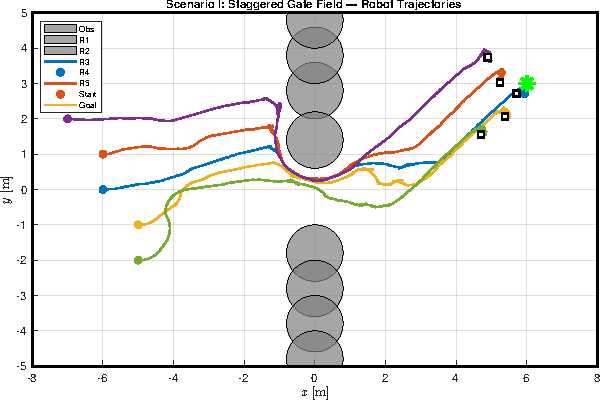
\includegraphics[width=\linewidth]{fig1_trajectory_gate}
  \caption{Scenario~I trajectory: Staggered Gate Field. The formation
  squeezes through the central gap ($x=0$) and re-establishes the
  $V$-shape beyond the obstacles.}
  \label{fig:traj_gate}
\end{figure}

\begin{figure}[!t]
  \centering
  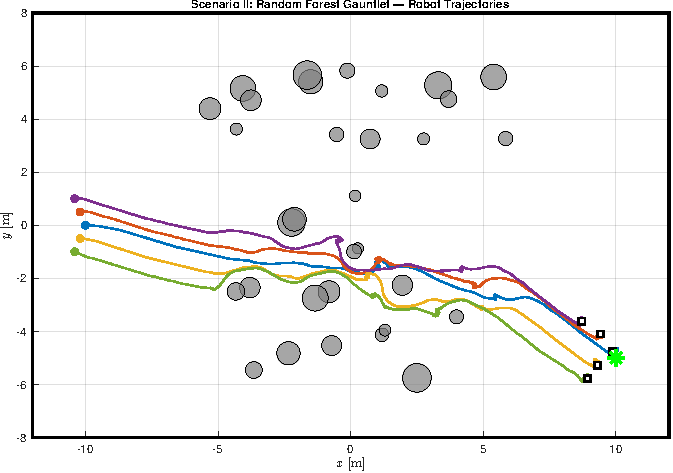
\includegraphics[width=\linewidth]{fig2_trajectory_forest}
  \caption{Scenario~II trajectory: Random Forest Gauntlet. The swarm
  navigates 32 randomly placed obstacles across the full 90~s simulation
  horizon while maintaining $\lambda_{2}>0$ and formation error below
  1.03~m peak.}
  \label{fig:traj_forest}
\end{figure}

\subsection{Formation Error Convergence}

Fig.~\ref{fig:form_error} shows the formation error norm $\|e(t)\|$ for
both scenarios.  In Scenario~I, the error begins at approximately
$\|e(0)\|\approx 1.34$~m as the swarm starts in a loose cluster and
converges rapidly as the distributed attractive forces pull agents toward
their $V$-shape targets.  A pronounced spike is observed as the formation
passes through the staggered gate at $x=0$: the dynamic squeeze
\eqnref{eq:squeeze} temporarily reduces $k_{\mathrm{form},i}$ to 10\% of
baseline, allowing the outer wing agents to decouple from the rigid geometry.
The error stabilizes at approximately $0.19$~m over the remainder of the
60~s simulation horizon.  Scenario~II exhibits a peak error of $1.02$~m and
a final error of $0.22$~m, with multiple transient spikes corresponding to
individual obstacle clusters and sustained convergence in the open regions
between them.  In both cases the error is non-zero but bounded during transit,
confirming that the squeeze mechanism successfully resolves the deadlock
without abandoning the formation entirely.

\begin{figure}[!t]
  \centering
  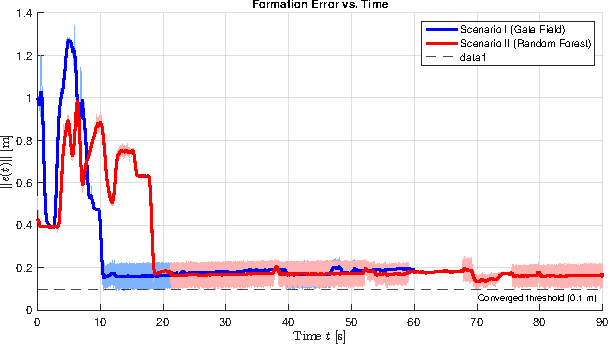
\includegraphics[width=\linewidth]{fig3_formation_error}
  \caption{Formation error $\|e(t)\|$ over time.  Peak errors of 1.34~m
  (Scenario~I) and 1.02~m (Scenario~II) occur during obstacle passages
  and reflect the dynamic formation squeeze activating; the error stabilizes
  below 0.22~m in the open field.}
  \label{fig:form_error}
\end{figure}

\subsection{Connectivity Preservation}

Fig.~\ref{fig:lambda2} plots $\lambda_{2}(L(t))$ for both scenarios.
The algebraic connectivity remains strictly positive throughout both trials,
confirming that no communication link was ever severed.  In Scenario~I,
$\lambda_{2}$ exhibits a shallow valley as agents compress through the
central gate, a direct consequence of agents temporarily approaching
$d_{\mathrm{th}}=1.8$~m.  The saturated tangent barrier \eqnref{eq:Fconn}
activates only during this brief window (when $d_{ij}>d_{\mathrm{safe}}$),
applying a restoring force that prevents any edge from reaching $d_{\mathrm{th}}$
and thus keeps $\lambda_{2}$ bounded away from zero.  In Scenario~II,
$\lambda_{2}$ fluctuates more broadly due to the stochastic obstacle layout,
but the minimum recorded values of $\lambda_{2}^{\min}=0.38$ (Scenario~I)
and $2.00$ (Scenario~II) remained strictly positive, validating the connectivity guarantee.

\begin{figure}[!t]
  \centering
  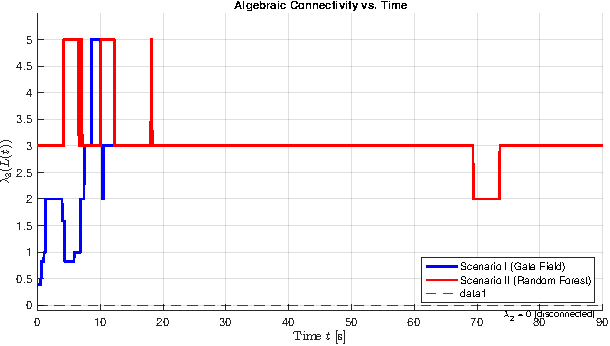
\includegraphics[width=\linewidth]{fig4_lambda2}
  \caption{Algebraic connectivity $\lambda_{2}(L(t))$. Both scenarios
  maintain $\lambda_{2}>0$ throughout (minimum values: $0.38$ in
  Scenario~I, $2.00$ in Scenario~II), confirming uninterrupted
  network connectivity.}
  \label{fig:lambda2}
\end{figure}

\subsection{Discussion}

The results demonstrate that the three proposed mechanisms interact
coherently.  The dynamic formation squeeze prevents the topological deadlock
that rigid APF formations would encounter at narrow passages.  The saturated
tangent barrier provides a \emph{reactive} connectivity restoring force that
incurs zero drag in the open field, unlike the continuous drag of classical
rational barriers \cite{panagou2016ITAC}.  The distributed target tracking
ensures that even if the network were transiently severed by an extreme
obstacle cluster, individual sub-swarms would self-navigate toward their
personal targets and reconnect naturally.

The high-frequency oscillation visible in the $\|e(t)\|$ plots is a
numerical artefact of the \emph{binary} adjacency model: as robots move
near $d_{\mathrm{th}}$, individual edges switch on and off between
timesteps, changing which pairs contribute to the error norm and producing
a sawtooth ripple around the true mean.  This is not noise in the control
sense — it does not reflect a physical force oscillation — but is rather a
consequence of the hard-threshold graph topology.  Replacing the binary
adjacency with a smooth, distance-weighted kernel would eliminate the
switching artefact at the cost of a more involved connectivity analysis.

The primary limitation of the current architecture is the reliance on a
continuous-time Lyapunov argument for a discrete-time implementation.  While
the penetration fail-safe and barrier cap provide practical safety guarantees,
a formal discrete-time Lyapunov proof would strengthen the theoretical
contribution.


\section{Conclusion}

This paper presented a decentralized formation controller for five unicycle
robots that simultaneously achieves $V$-shape formation stabilization,
static obstacle avoidance, and strict communication connectivity preservation
in cluttered two-dimensional environments.  The nonholonomic kinematic
constraint was resolved via feedback linearization through a look-ahead
point, mapping each unicycle onto a fully actuated virtual integrator and
enabling direct application of gradient-descent control laws.  Three
complementary mechanisms were introduced: a \emph{dynamic formation squeeze}
that adaptively relaxes the rigid formation geometry in narrow corridors; a
\emph{saturated tangent barrier} that incurs zero connectivity drag in the
open field and activates only when an inter-agent link approaches the
communication threshold; and \emph{leaderless distributed target tracking}
that enables automatic network self-recovery after transient topological
splits.  A Lyapunov argument demonstrated that the safe connected invariant
set $\Omega=\{\mathbf{p}_{v}\in\scr{W}_{\mathrm{free}}^{N}:\lambda_{2}(L)>0\}$
is forward invariant under the proposed control law, and the five APF
hyperparameters were tuned via Bayesian optimization to ensure
generalizability across diverse obstacle environments.

Simulations in a structured staggered gate field and a random obstacle
forest confirmed successful goal acquisition with zero collisions.  The
algebraic connectivity remained strictly positive throughout all trials
($\lambda_{2}^{\min}=0.38$ in Scenario~I and $2.00$ in Scenario~II),
validating the connectivity guarantee in practice.

Three directions are identified for future work.  First, extending the
framework to dynamic obstacles and moving agents is a natural next step
toward real deployment.  Second, replacing the binary adjacency graph with
a smooth distance-weighted kernel would eliminate the edge-switching
artefact observed in the formation error and enable a cleaner barrier
potential formulation.  Third, a formal discrete-time Lyapunov proof
is needed to close the gap between the continuous-time stability argument
and the Euler-integrated implementation.


\bibliographystyle{unsrt}
\bibliography{MAAC_Paper}


\end{document}
